\documentclass[letterpaper,12pt]{article}
\usepackage{array}
\usepackage{threeparttable}
\usepackage{geometry}
\geometry{letterpaper,tmargin=1in,bmargin=1in,lmargin=1.25in,rmargin=1.25in}
\usepackage{fancyhdr,lastpage}
\pagestyle{fancy}
\lhead{}
\chead{}
\rhead{}
\lfoot{}
\cfoot{}
\rfoot{\footnotesize\textsl{Page \thepage\ of \pageref{LastPage}}}
\renewcommand\headrulewidth{0pt}
\renewcommand\footrulewidth{0pt}
\usepackage[format=hang,font=normalsize,labelfont=bf]{caption}
\usepackage{listings}
\lstset{frame=single,
  showstringspaces=false,
  columns=flexible,
  basicstyle={\small\ttfamily},
  numbers=none,
  breaklines=true,
  breakatwhitespace=true
  tabsize=3
}
\usepackage{amsmath}
\usepackage{amssymb}
\usepackage{amsthm}
\usepackage{harvard}
\usepackage{setspace}
\usepackage{float,color}
\usepackage[pdftex]{graphicx}
\usepackage{hyperref}
\hypersetup{colorlinks,linkcolor=red,urlcolor=blue}
\theoremstyle{definition}
\newtheorem{theorem}{Theorem}
\newtheorem{acknowledgement}[theorem]{Acknowledgement}
\newtheorem{algorithm}[theorem]{Algorithm}
\newtheorem{axiom}[theorem]{Axiom}
\newtheorem{case}[theorem]{Case}
\newtheorem{claim}[theorem]{Claim}
\newtheorem{conclusion}[theorem]{Conclusion}
\newtheorem{condition}[theorem]{Condition}
\newtheorem{conjecture}[theorem]{Conjecture}
\newtheorem{corollary}[theorem]{Corollary}
\newtheorem{criterion}[theorem]{Criterion}
\newtheorem{definition}[theorem]{Definition}
\newtheorem{derivation}{Derivation} % Number derivations on their own
\newtheorem{example}[theorem]{Example}
\newtheorem{exercise}[theorem]{Exercise}
\newtheorem{lemma}[theorem]{Lemma}
\newtheorem{notation}[theorem]{Notation}
\newtheorem{problem}[theorem]{Problem}
\newtheorem{proposition}{Proposition} % Number propositions on their own
\newtheorem{remark}[theorem]{Remark}
\newtheorem{solution}[theorem]{Solution}
\newtheorem{summary}[theorem]{Summary}
%\numberwithin{equation}{section}
\bibliographystyle{aer}
\newcommand\ve{\varepsilon}
\newcommand\boldline{\arrayrulewidth{1pt}\hline}


\begin{document}

\begin{flushleft}
  \textbf{\large{Problem Set \#1}} \\
  Econ Theory, Jason Debacker \\
  Alex Weinberg
\end{flushleft}

\vspace{5mm}



\noindent\textbf{Problem 1} ~\\
Consider the problem of the owner of an oil field. The owner has B barrels of oil. She can
sell these barrels at price pt at time t. Her objective is to maximize the discounted present
value of sales of oil - we’ll assume there are no extraction costs. The owner discounts the
future at a rate given by 1/1+r (where r is the real interest rate and assumed to be constant). Answer the following: \\~\\
1. What are the state variables? \\
2. What are the control variables? \\
3. What does the transition equation look like? \\
4. Write down the sequence problem of the owner. Write down the Bellman equation. \\
5. What does the owner’s Euler equation like? \\
6. What would the solution of the problem look like if pt+1 = pt for all t? What would the solution look like if pt+1 > (1 + r)pt for all t? What is the condition on the path of prices necessary for an interior solution (where the owner will extract some, but not all, of the oil)?


\begin{solution} ~\\
  \begin{enumerate}
  \item The state variable is B. The prices r,$p_t$ are given exogenously.
  \item Control variables are B' (oil to save) and b (oil to sell today)
  \item Transition equation is B' = B - b
  \item Sequence problem is: \[ \max \sum_{i=0}^\infty \frac{b_tp_t}{(1+r)^t} \] \\
  Bellman equation is:
  \[ V(B) = p_tb_t + \quad \frac{1}{1+r} V(B')\]
  \item Euler equation is: \[ p_t = \frac{1}{1+r}p_{t+1}
  \]
  \item
  \begin{itemize}
    \item If $p_{t+1}=p_t=p \quad \forall t$ then the owner will sell all oil today.
    \item If $p_{t+1} > (1+r) p_t \quad \forall t$ then she always saves all B til tomorrow.
    \item $p_t = \frac{1}{1+r}p_{t+1}$ is the necessary condition for the owner to be indifferent between extracting today and extracting tomorrow.
  \end{itemize}
  \end{enumerate}
\end{solution}
%-------------------------------------

\noindent\textbf{Problem 2} ~\\
The Neoclassical Growth Model is a workhorse model in macroeconomics. The problem for the social planner is to maximize the discounted expected utility for agents in the economy:
∞
 maxE  βtu(c) (1) {c}∞0 t
t=0 t=0 1
The resource constraint is given as:
yt = ct + it (2) The law of motion for the capital stock is:
kt+1 =(1−δ)kt +it (3) Output is determined by the aggregate production function:
yt = ztktα (4) Assume that zt is stochastic. In particular, it is an i.i.d. process distributed as ln(z) ∼
N(0,σz).

\begin{solution} ~\\
  \begin{enumerate}
  \item State variable is $k_t, z_t$
  \item Control variables are $c_t,i_t$ can reduce to just $c_t$
  \item $V(k_t,z_t) = u(c_t) + \beta E_t[V(k_{t+1},z_{t+1}) \mid z_{t}]$ \\ s.t.
  \end{enumerate}
  \begin{gather}
    y_t = c_t + i_t \\
    k_{t+1} = (1- \delta)k_t + i_t \\
    y_t = z_tk_t^\alpha
  \end{gather}
  \item \lstinputlisting[language=python]{ncg.py}
  \begin{figure}[htb]\centering\captionsetup{width=4.0in}
    \caption{\textbf{Great example figure}}\label{}
    \fbox{\resizebox{4.0in}{3.0in}{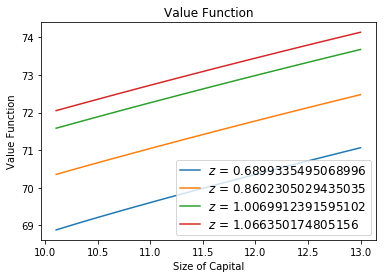
\includegraphics{one.png}}}
  \end{figure}
  \begin{figure}[htb]\centering\captionsetup{width=4.0in}
    \caption{\textbf{Great example figure}}\label{}
    \fbox{\resizebox{4.0in}{3.0in}{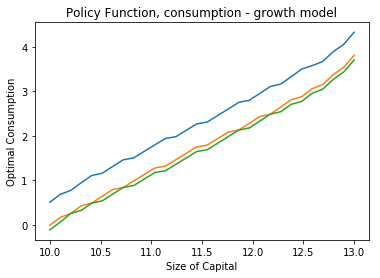
\includegraphics{two.png}}}
  \end{figure}
  \begin{figure}[htb]\centering\captionsetup{width=4.0in}
    \caption{\textbf{Great example figure}}\label{}
    \fbox{\resizebox{4.0in}{3.0in}{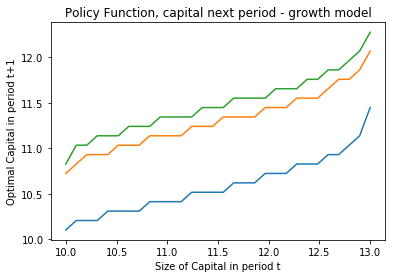
\includegraphics{three.png}}}
  \end{figure}
\end{solution}

\begin{solution}
Change rho = 0.8 in above.
$$V(w) = \max\{V^U(w), V^J(w)\}$$
where: $$V^U(w)= b + \beta E V(w)$$ and $$V^J(w) = E_0 \sum_{t=0}^{\infty} \beta^t w = \frac{w}{1 - \beta} $$
\begin{figure}[htb]\centering\captionsetup{width=4.0in}
  \caption{\textbf{Great example figure}}\label{}
  \fbox{\resizebox{4.0in}{3.0in}{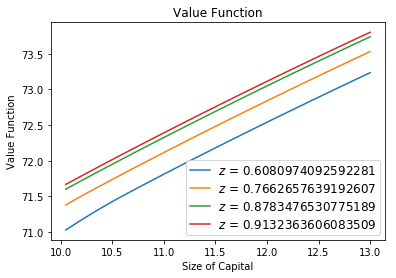
\includegraphics{1.png}}}
\end{figure}
\begin{figure}[htb]\centering\captionsetup{width=4.0in}
  \caption{\textbf{Great example figure}}\label{}
  \fbox{\resizebox{4.0in}{3.0in}{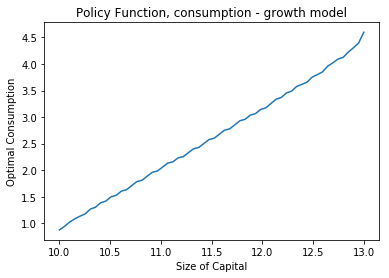
\includegraphics{2.png}}}
\end{figure}
\begin{figure}[htb]\centering\captionsetup{width=4.0in}
  \caption{\textbf{Great example figure}}\label{}
  \fbox{\resizebox{4.0in}{3.0in}{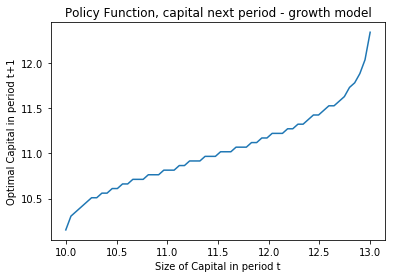
\includegraphics{3.png}}}
\end{figure}
\end{solution}

\newpage
\begin{solution}
See LaborDP.ipyb for answers and code.
\end{solution}
%-----------------------------
\end{document}
